\begin{tikzpicture}[
    declare function={
      msea(\k,\t)  = 2/(\t-\k);},                       % MSE(s^2)/sigma^4
    declare function={
      msem(\k,\t)  = (2*(\t-\k)+\k*\k)/(\t*\t);}        % MSE(MV)/sigma^4
]
\begin{axis}[
  width = 11cm, height = 6.5cm,
  xlabel = {Nombre de régresseurs $K$},
  ylabel = {$\nicefrac{MSE}{\sigma_{\varepsilon}^4}$},
  domain = 1:12, samples = 12,
  xtick = {1,2,...,12},
  legend cell align = left,
  legend style = {at={(0.02,0.98)}, anchor=north west},
  grid = major, grid style = {gray!20}]

  \addplot[very thick, blue!70!black, mark=*, mark size=1.4pt] {msea(x,50)};
  \addlegendentry{$MSE(s^2)$}

  \addplot[very thick, red!75!black, mark=square*, mark size=1.4pt] {msem(x,50)};
  \addlegendentry{$MSE(\hat\sigma_{\varepsilon}^2)$, maximum de vraisemblance}

  % Le croisement : au-delà de K = 4, s^2 l'emporte.
  \draw[dashed, black!55] (axis cs:4,0) -- (axis cs:4,0.06);
  \node[anchor=south, font=\footnotesize, black!70] at (axis cs:4,0.0605) {$K=4$};

\end{axis}
\end{tikzpicture}
